% Cluster analysis
\chapter{Clustering analysis} \label{s:ap:cs}


\section{non-PCA} \label{s:ap:non-pca}


\begin{figure}[!h]
    \captionsetup[subfigure]{justification=Centering}
    \centering
    \begin{subfigure}[!t]{0.6\textwidth}
        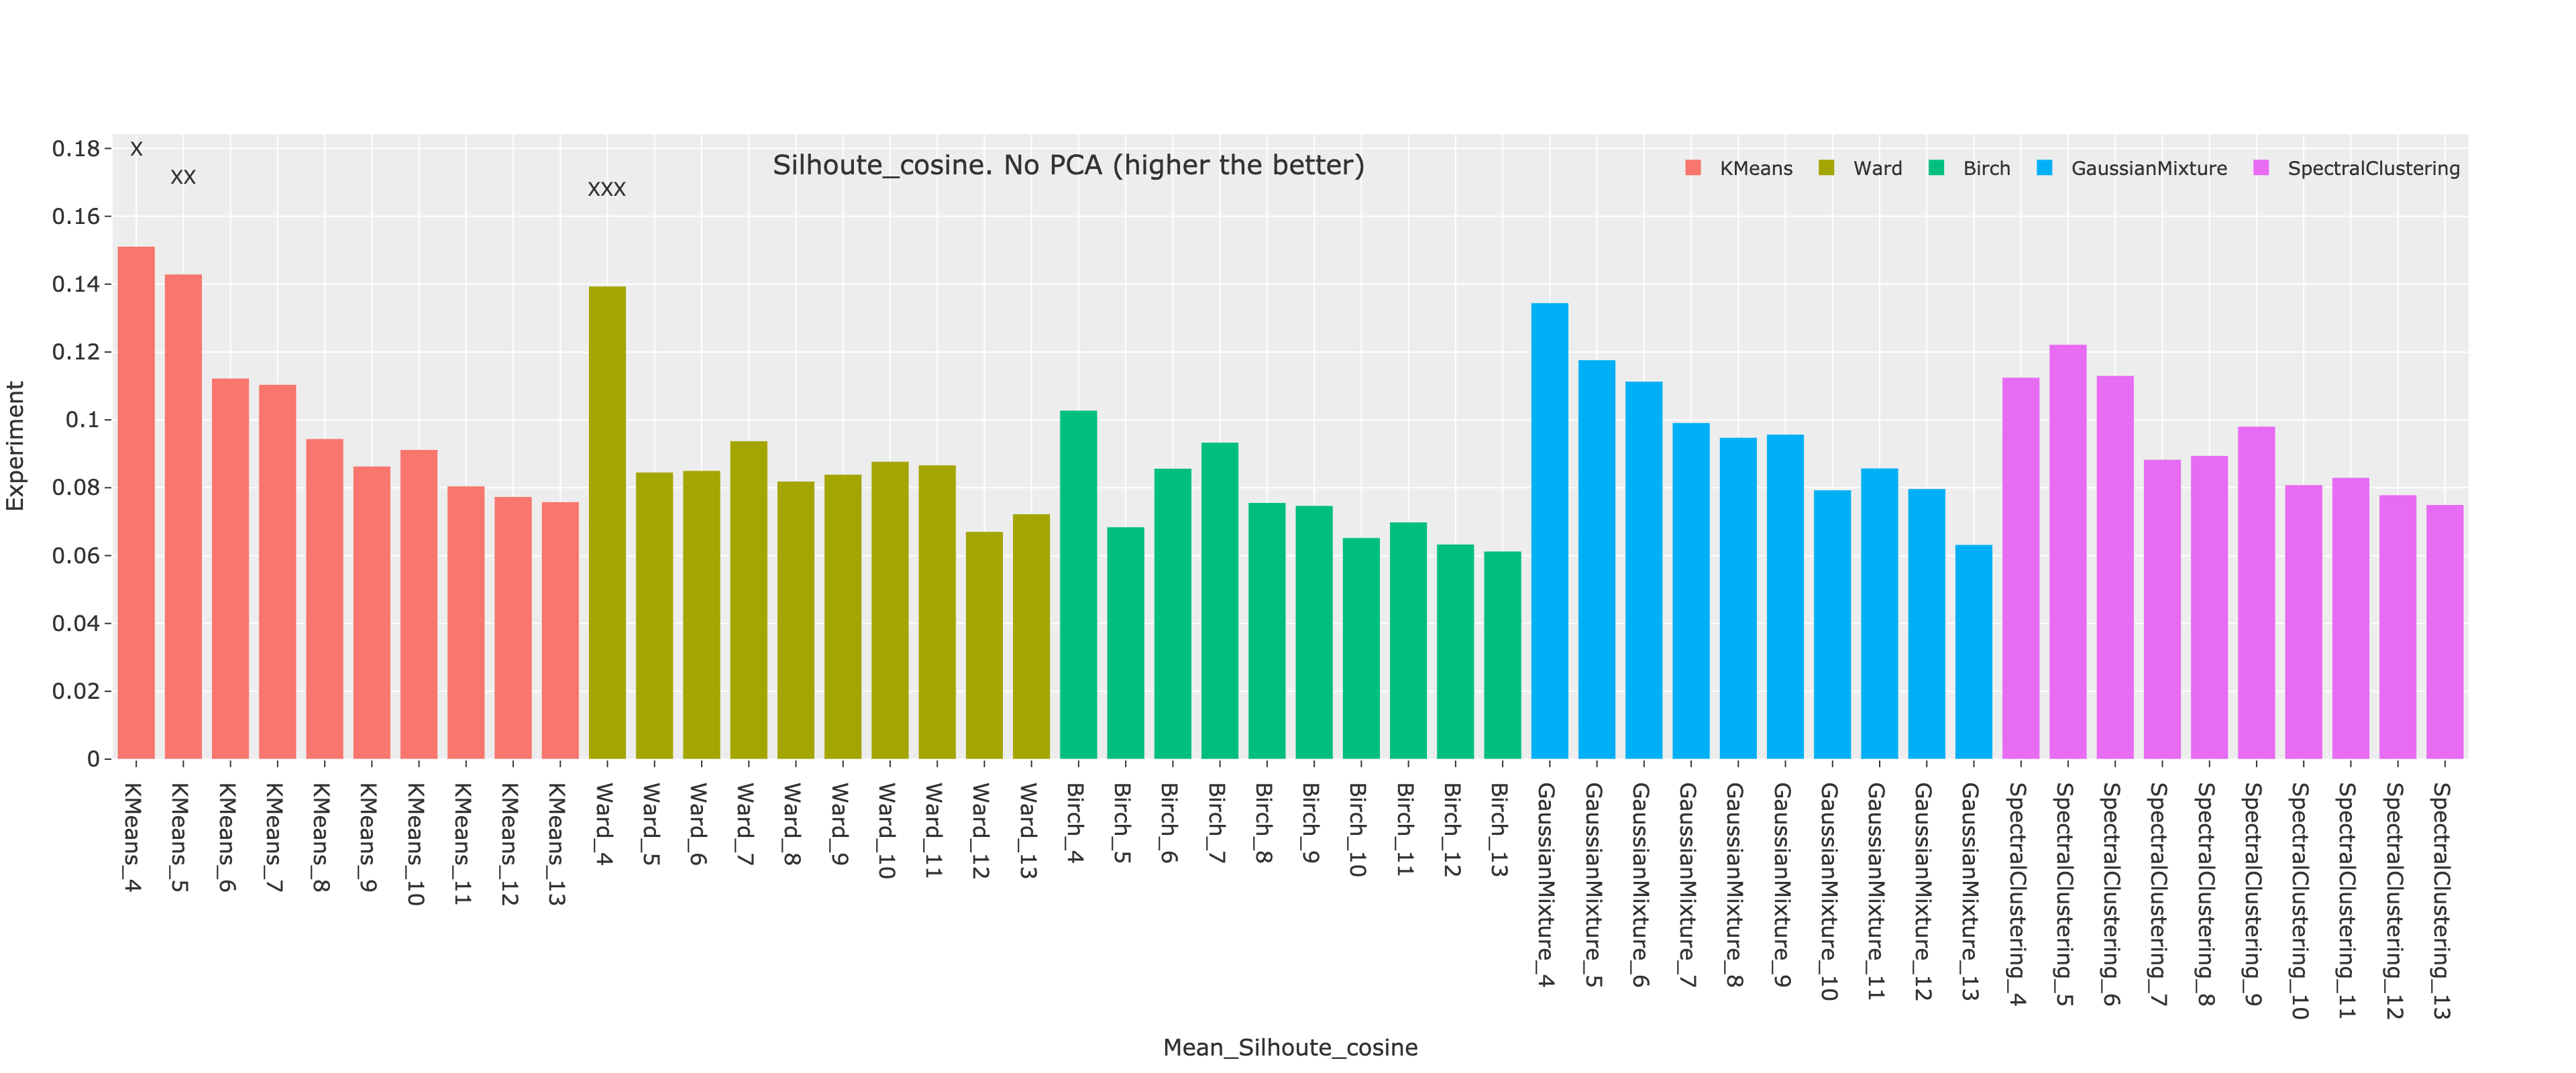
\includegraphics[width=\textwidth]{Sections/ClusteringAnalysis/Resources/cs_top3/nonPCA/non_PCA_top3_Silhoute_cosine.png}
        \caption{Silhouette using cosine distance}
        \label{fig:ap:cosine}
    \end{subfigure}
    \centering
    \begin{subfigure}[!t]{0.6\textwidth}
        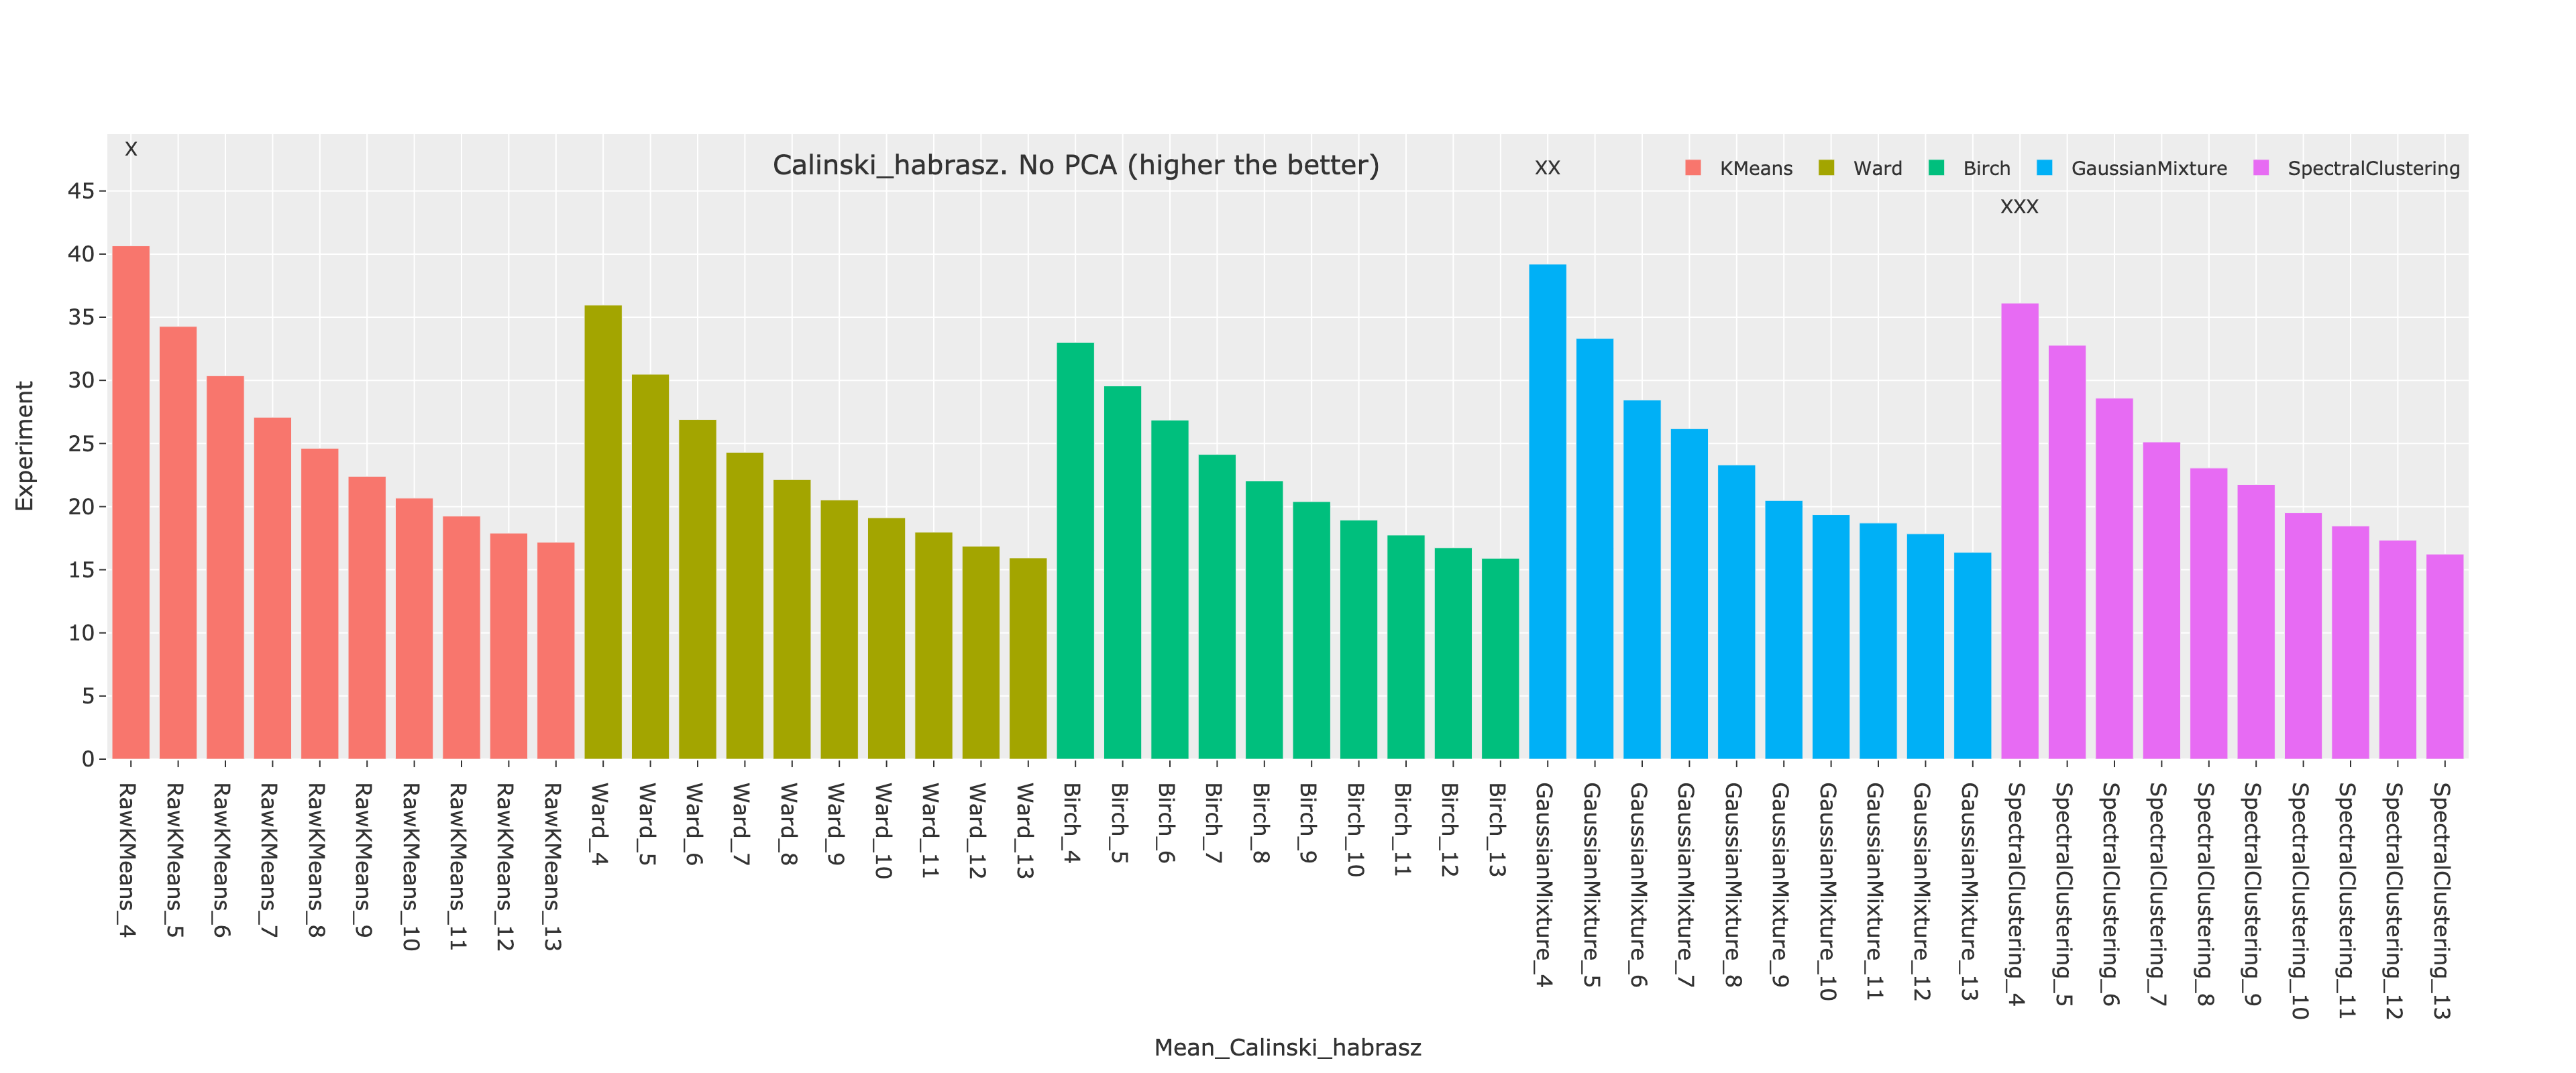
\includegraphics[width=\textwidth]{Sections/ClusteringAnalysis/Resources/cs_top3/nonPCA/non_PCA_top3_Calinski_habrasz.png}
        \caption{Calinski Harabasz}
        \label{fig:ap:cal_hab}
    \end{subfigure}
    \centering
    \begin{subfigure}[!t]{0.6\textwidth}
        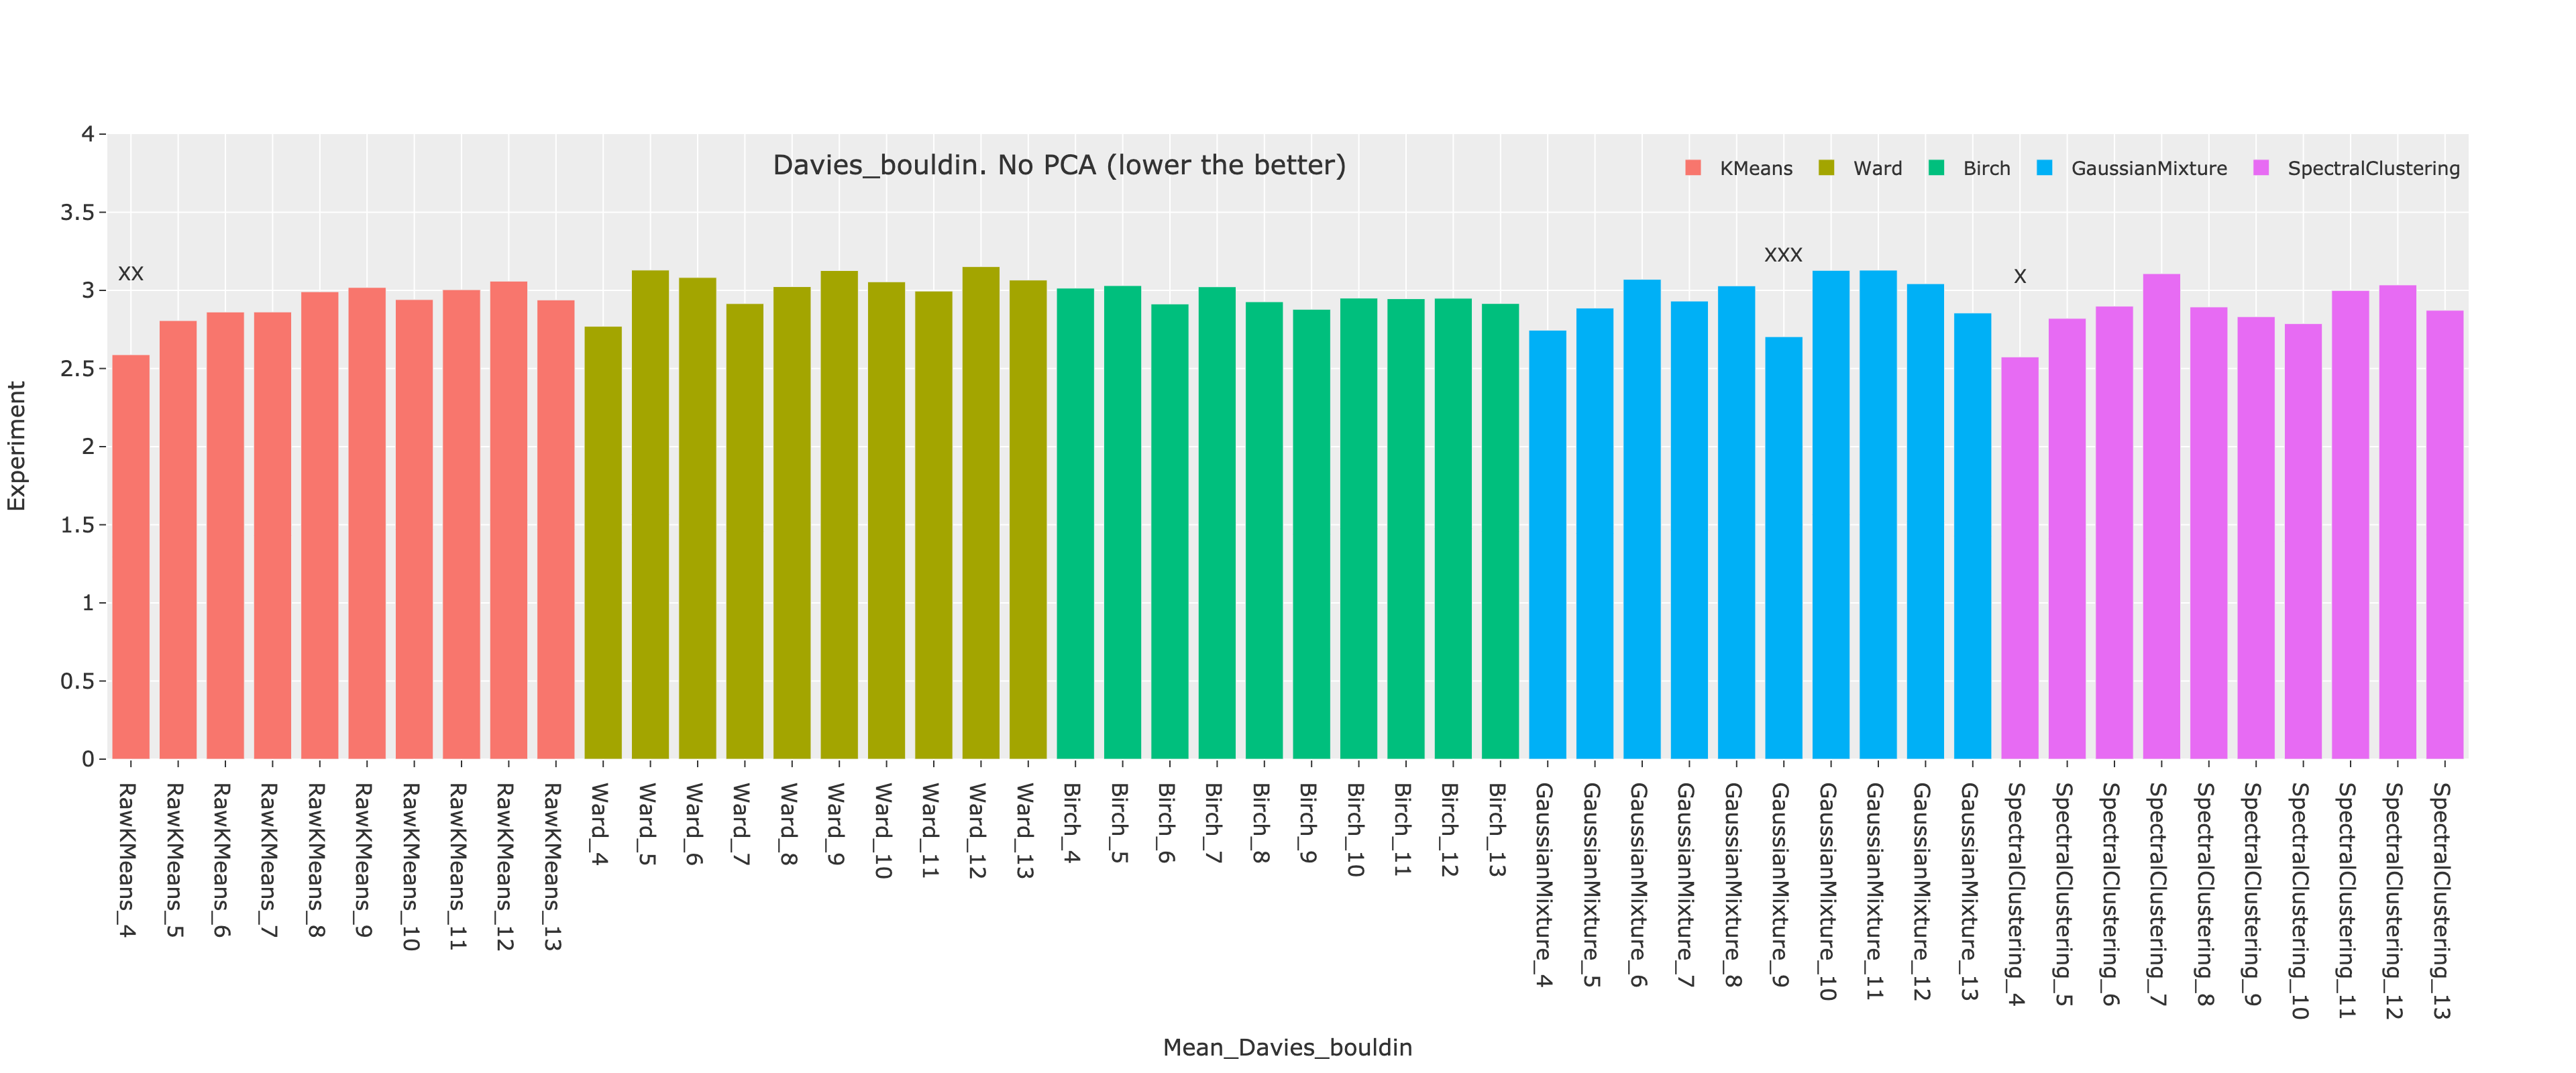
\includegraphics[width=\textwidth]{Sections/ClusteringAnalysis/Resources/cs_top3/nonPCA/non_PCA_top3_Davies_bouldin.png}
        \caption{Davies Bouldin}
        \label{fig:ap:dav_boul}
    \end{subfigure}
    \caption{The means of the three cluster metrics introduced in \cref{s:lit:clustering_metrics}: Silhouette (cosine), Calinski Harabasz and Davies Bouldin. Each of them asses different aspects of clustering and are used to determined the right clustering model for the MIBC cohort from TCGA. The gene expression is processed according to \cref{s:cs:methods} and data was not PCA transformed.}
    \label{fig:ap:non_pca_metrics}
\end{figure}


\section{GSEA - Hallmarks database} \label{s:ap:cs:gsea_ne}

\subsection{LumInf}

\begin{figure}[H]    
    \centering
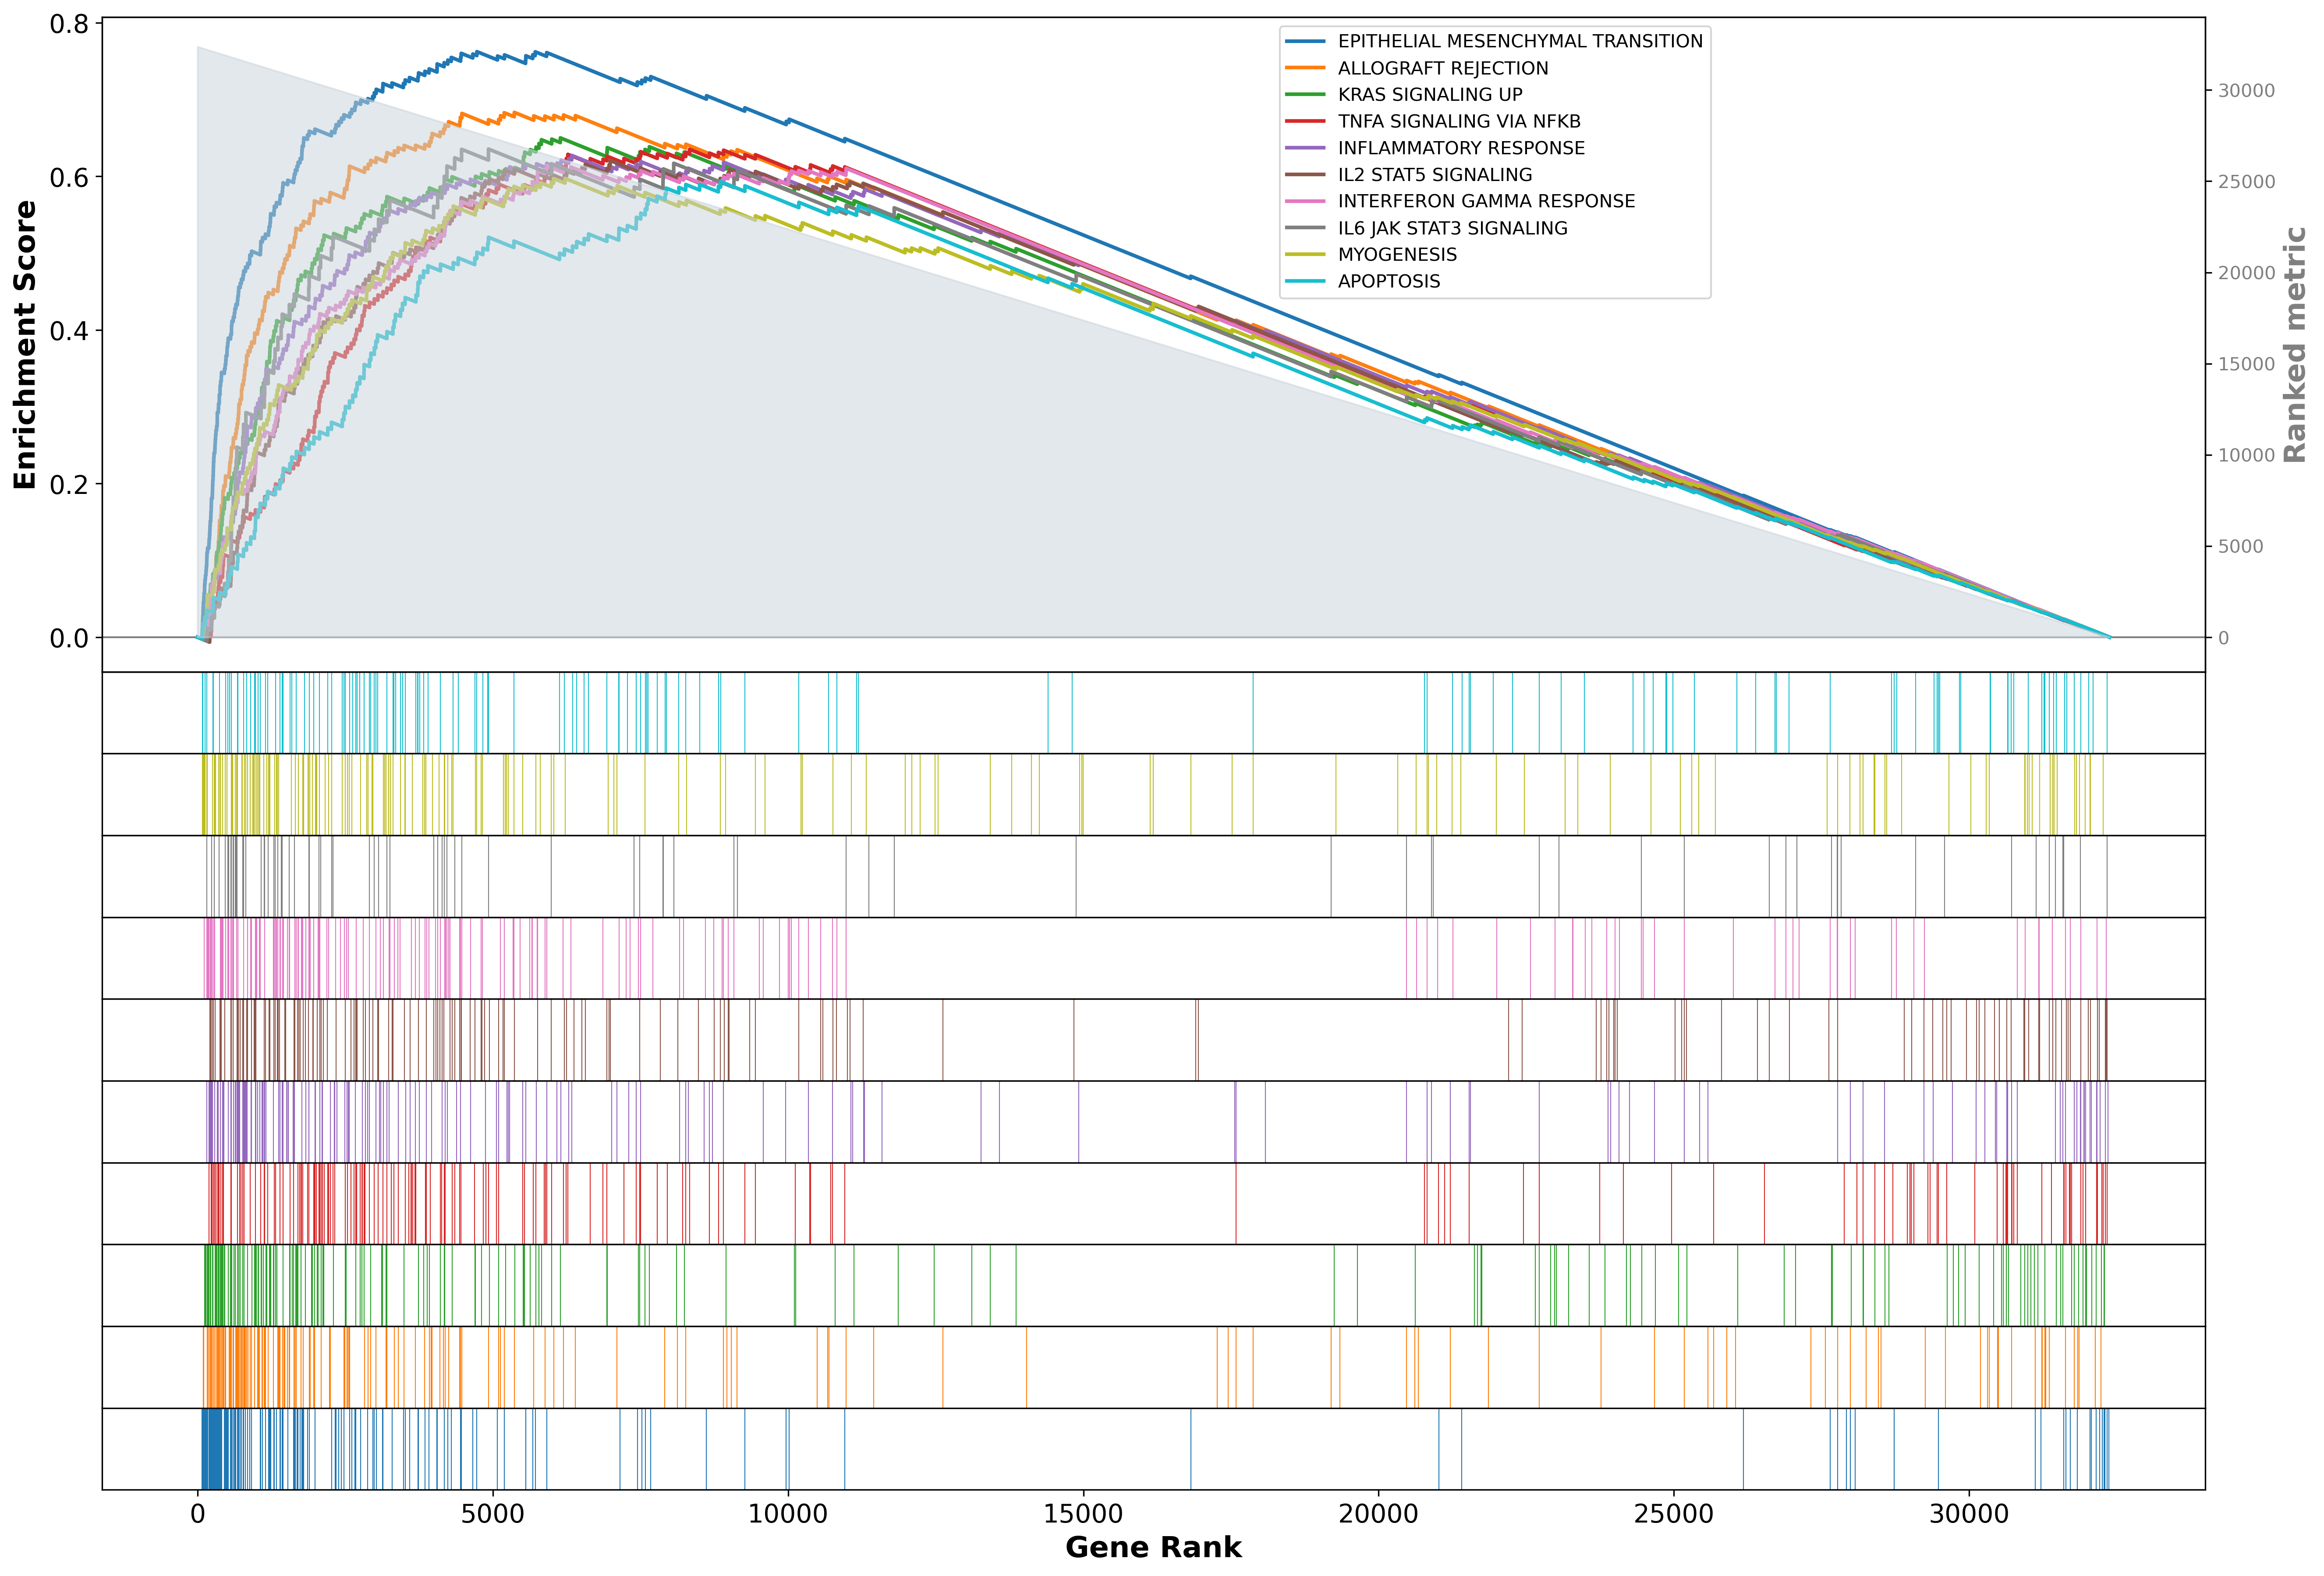
\includegraphics[width=1.0\textwidth,keepaspectratio]{Sections/ClusteringAnalysis/Resources/discussion/other_groups/lumInf_hallmark_10_top.png}
    \caption{For the Luminal Infiltrated group derived in \cref{s:cs:bio_interp} and accompanying the analysis in \cref{s:cs:lumInf_interp}. The top 10 terms of running GSEA on the Hallmark database. The ranking is using the pi plot from \cref{fig:cs:lumInf_pi}}
    \label{fig:ap:cs:gsea_lumInf_hallmark}
\end{figure}


\subsection{LumP}


\begin{figure}[H]    
    \centering
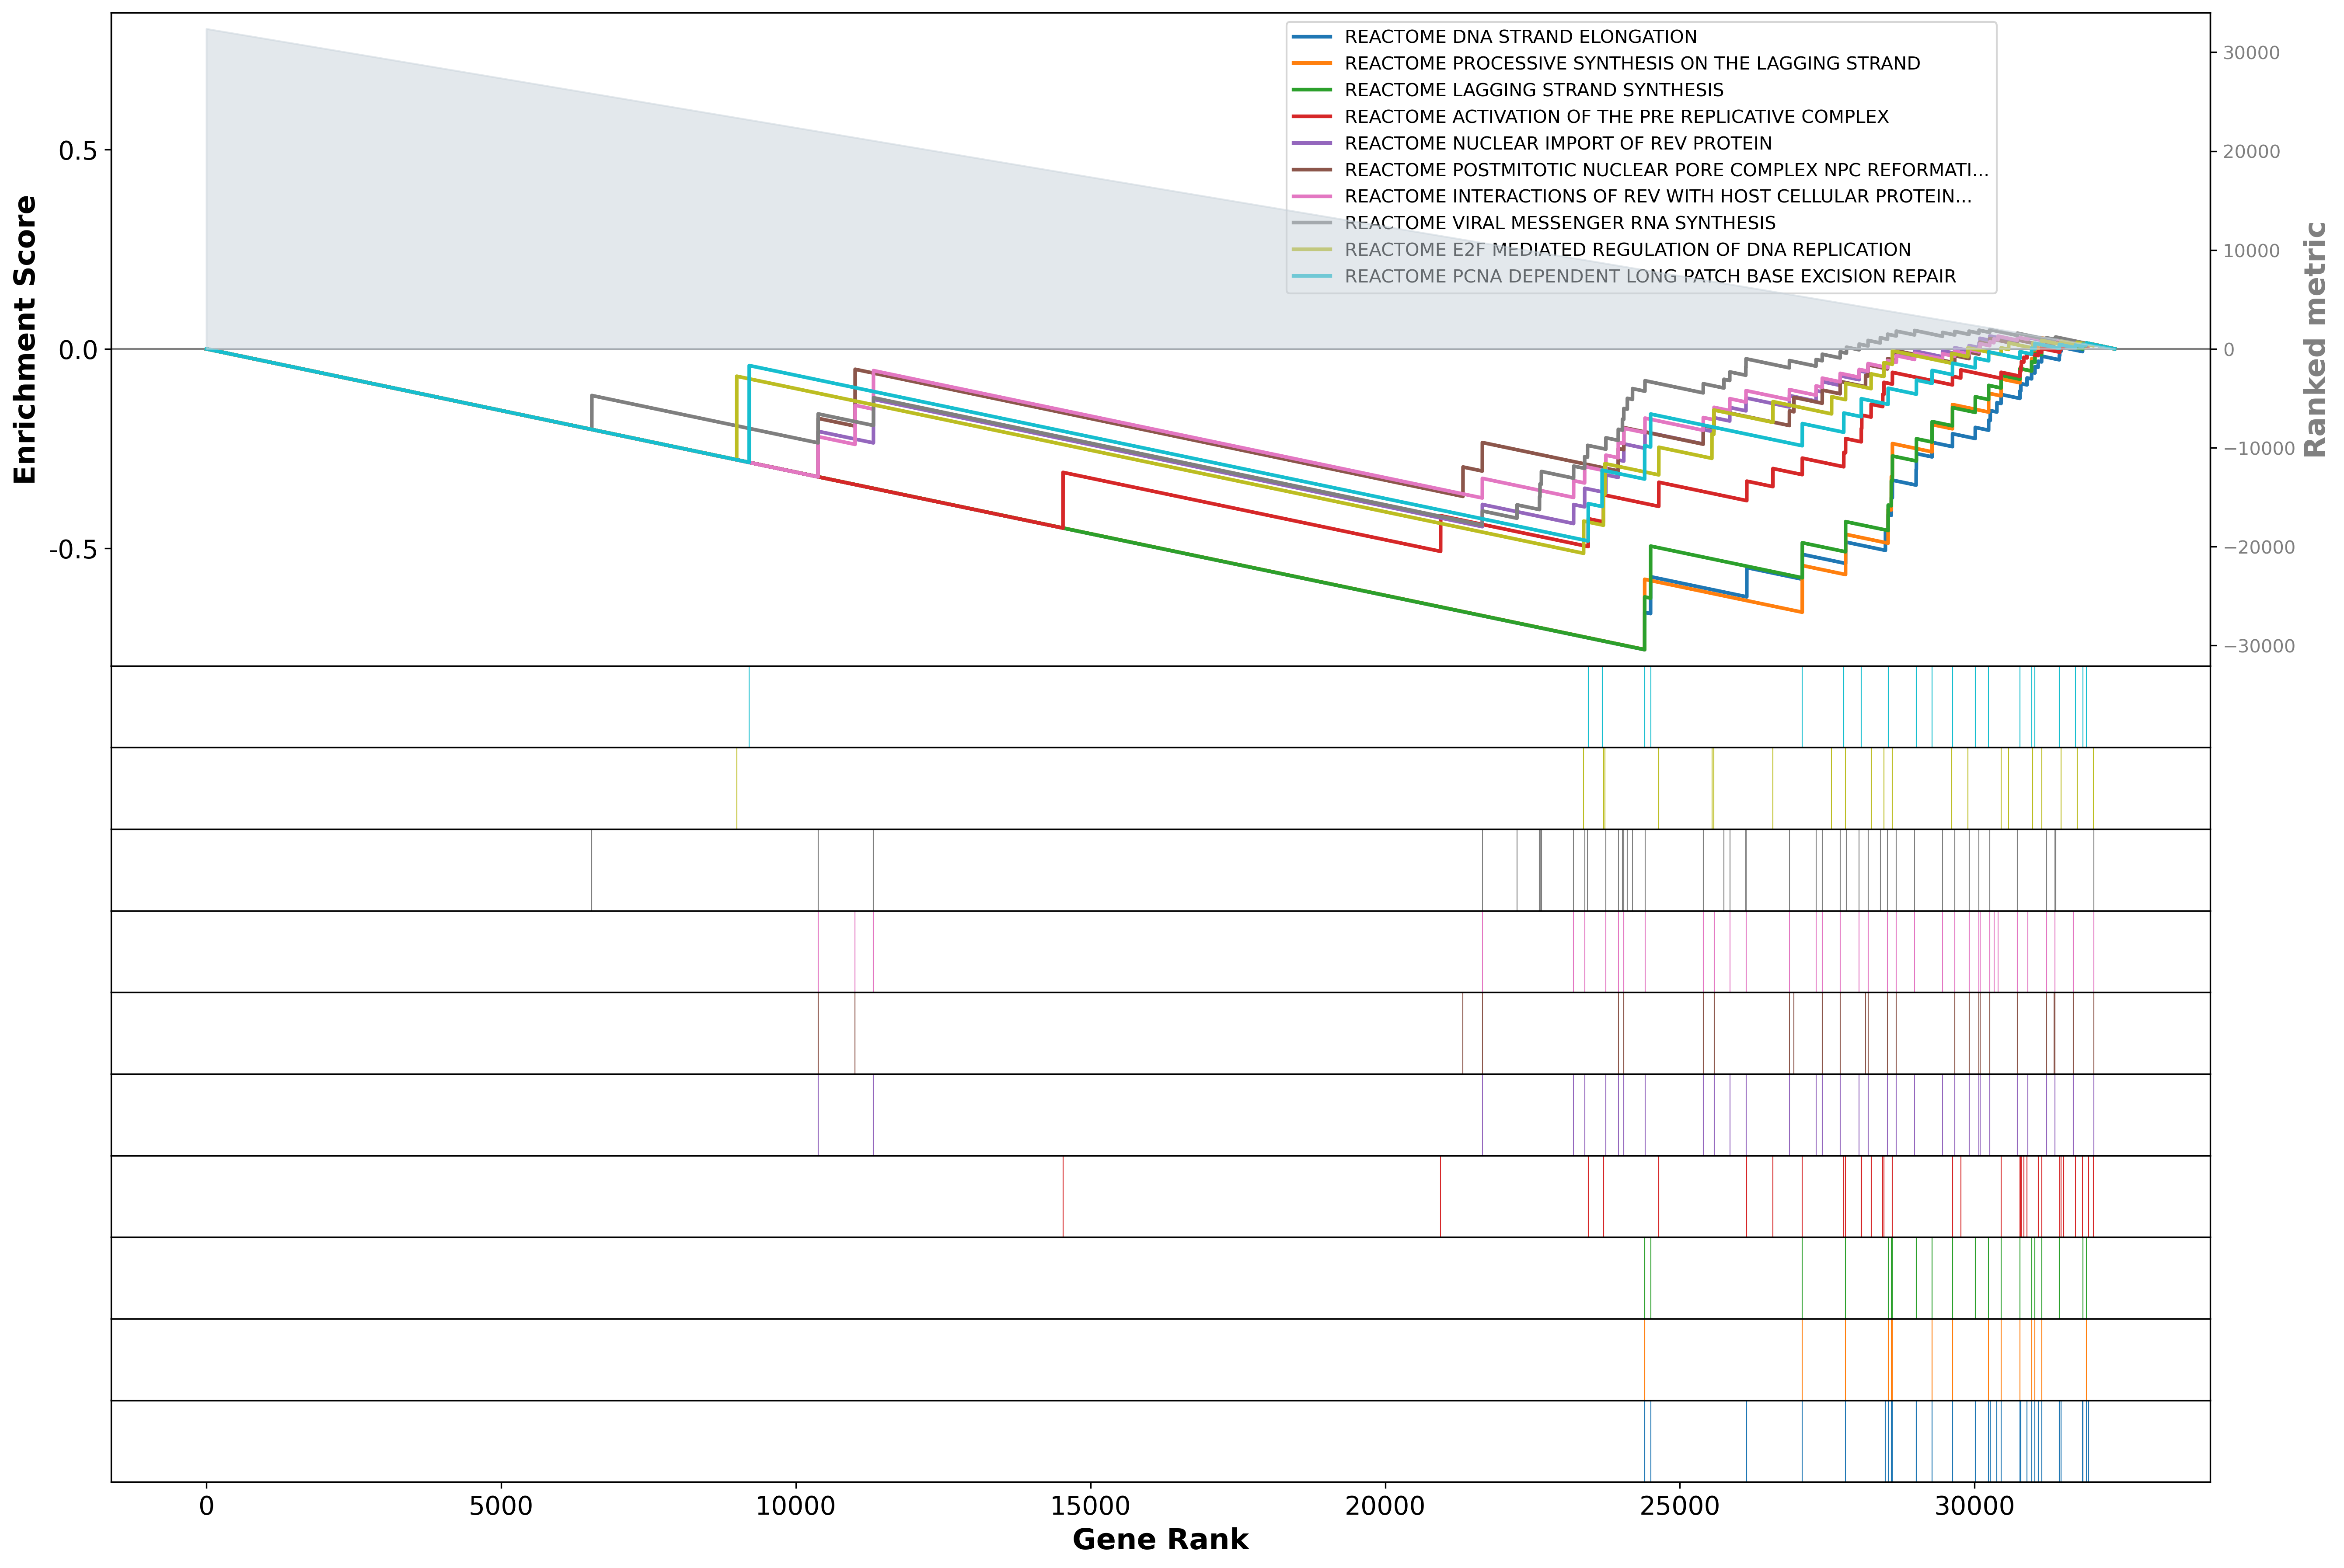
\includegraphics[width=1.0\textwidth,keepaspectratio]{Sections/ClusteringAnalysis/Resources/discussion/other_groups/lumP2_hallmark_10_top.png}
     \caption{For the Luminal Papillary group derived in \cref{s:cs:bio_interp} and accompanying the analysis in \cref{s:cs:lumP_interp}. The top 10 terms of running GSEA on the Hallmark database. The ranking is using the pi plot from \cref{fig:cs:lumP_pi}}
    \label{fig:ap:cs:gsea_lump_hallmark}
\end{figure}


\subsection{NE-like}


\begin{figure}[H]    
    \centering
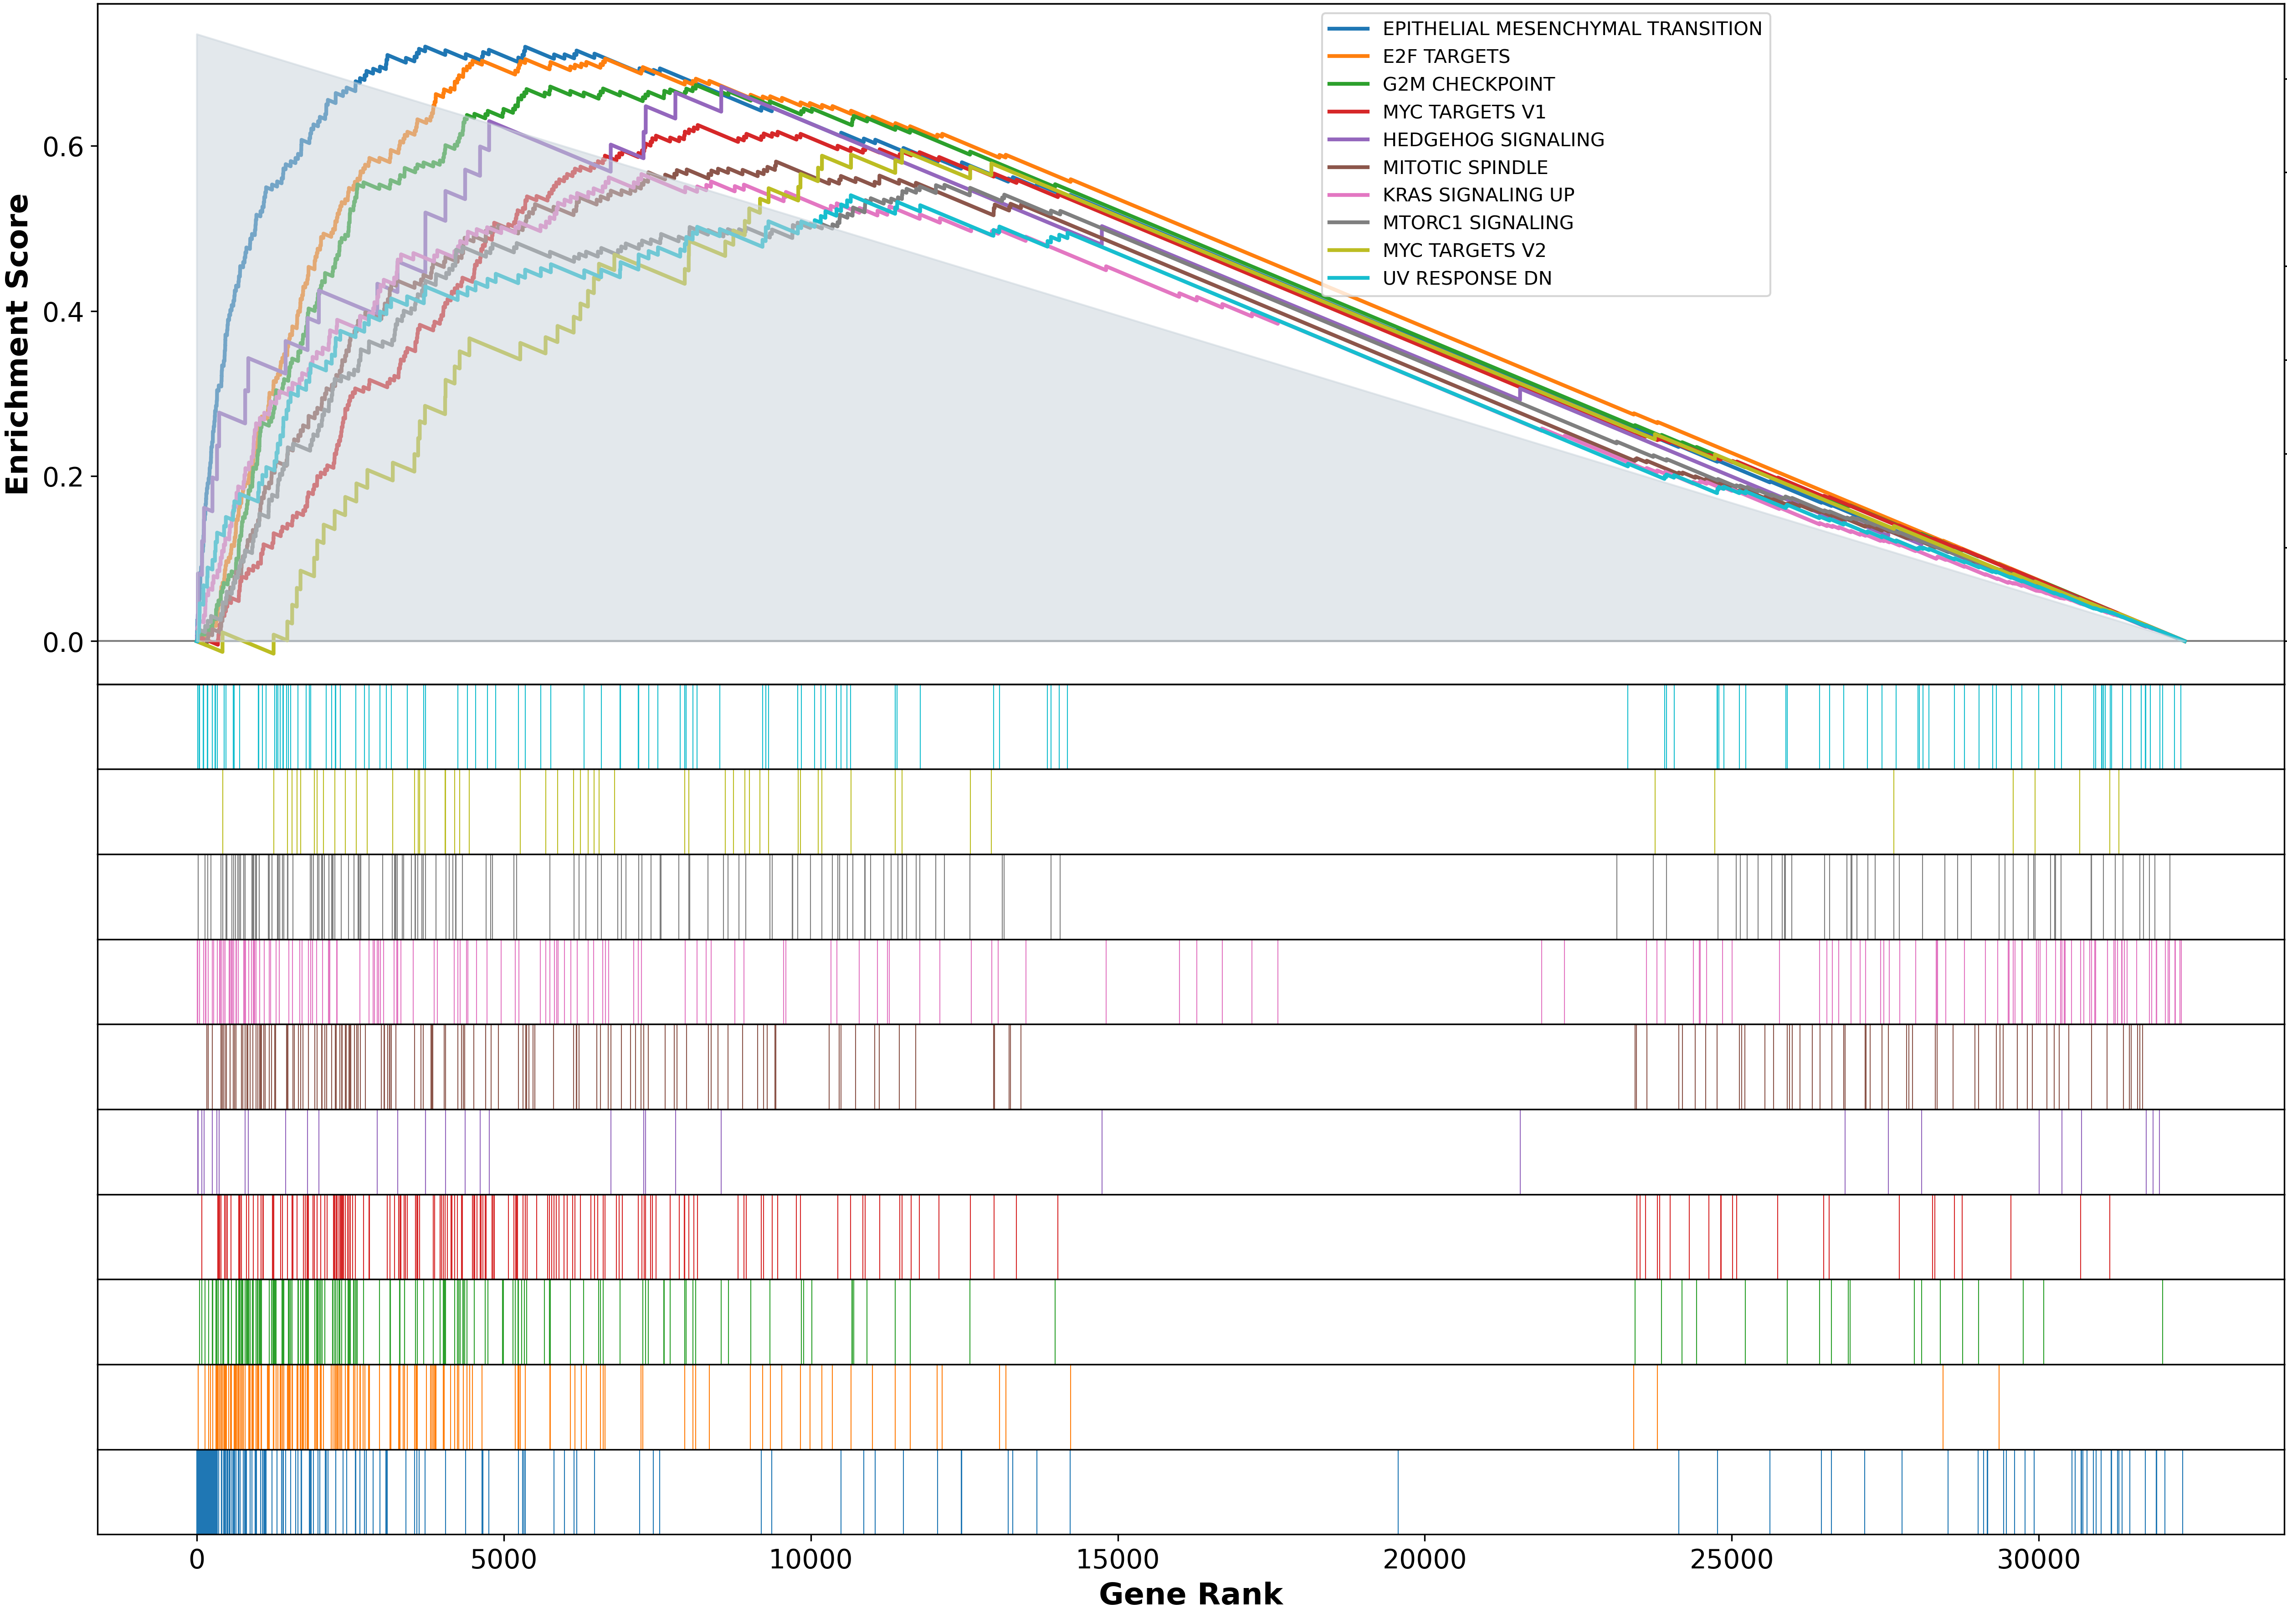
\includegraphics[width=1.0\textwidth,keepaspectratio]{Sections/ClusteringAnalysis/Resources/discussion/other_groups/ne2_hallmark_10_top.png}
     \caption{For the Neuroendocrine-like group derived in \cref{s:cs:bio_interp} and accompanying the analysis in \cref{s:cs:ne_interp}. The top 10 terms of running GSEA on the Hallmark database. The ranking is using the pi plot from \cref{fig:cs:ne_pi}}
    \label{fig:ap:cs:gsea_ne_hallmark}
\end{figure}
